\documentclass[a4paper, 12pt]{scrartcl}

\usepackage{scrpage2}
\usepackage[left=2.5cm,right=2.5cm, top=3cm, bottom=4cm]{geometry}
\usepackage[utf8]{inputenc}
\usepackage[ngerman]{babel}
\usepackage[T1]{fontenc}
\usepackage{amsmath}
\usepackage{amssymb}
\usepackage{amsfonts}

\usepackage{graphicx}

\usepackage{float}
\usepackage{adjustbox}
\usepackage{hyperref}
\usepackage{textcomp}

%\usepackage{enumerate}
\usepackage[shortlabels]{enumitem}

% Einrücken verhindern
\setlength{\parindent}{0em} 


\begin{document}


\begin{titlepage}
	\centering
	{\Huge\bfseries Versuchsprotokoll\par}
	\vspace{2cm}
	{\scshape\LARGE Mechanik \par}
	\vspace{1cm}
	{\Large Pendel- und Fallexperiment zur Bestimmung der Erdbeschleunigung\par}
	\vfill
	{\large\itshape Simon Schwarz und Marius Ising\par}

	\vfill
\end{titlepage}

\tableofcontents
\newpage

\section{Erdbeschleunigung mit dem Fallexperiment}


\subsection{Versuchsbeschreibung}

Das Ziel des folgenden Versuchs ist die Bestimmung der Erdbeschleunigung $g$. Für eine gleichmäßig beschleunigte Bewegung gilt die Differentialgleichung
$$\ddot s = \frac{d^2s}{dt^2} = a = \mathrm{const}.$$
Durch zweifache Integration erhält man das Weg-Zeit-Gesetz dieser Bewegung
$$s(t) = s_0 + v_0t + \frac a2 t^2.$$
Dabei ist $v_0$ die Anfangsgeschwindigkeit und $s_0$ der anfängliche Weg zum Zeitpunkt $t=0$. Für den betrachteten freien Fall ist dabei die Beschleunigung $a$ gleich der Erdbeschleunigung $g$. Aufgrund der geringen auftretenden Geschwindigkeiten werden zudem Luftreibungseffekte vernachlässigt. Durch eine Weg-Zeit-Messung lässt sich somit $g$ bestimmen.


\subsection{Versuchsaufbau}

\begin{figure}[h]
	\centering
	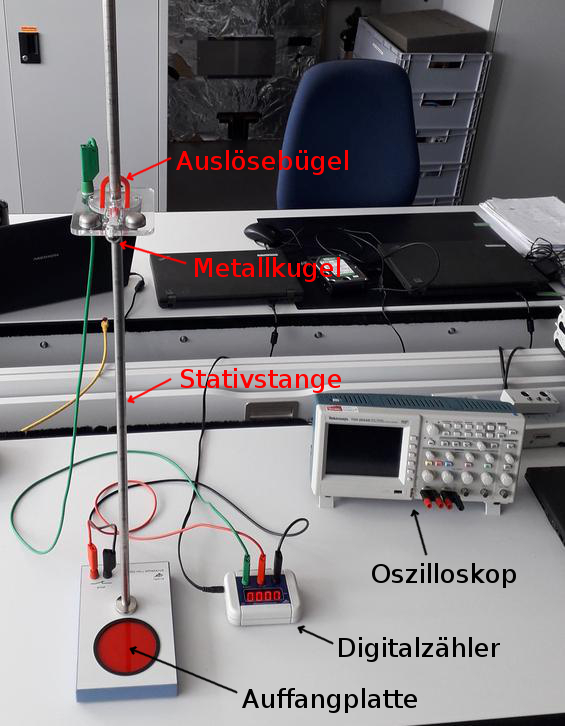
\includegraphics{bilder/Aufbau_fF_be.jpg}
	\caption{Versuchsaufbau}
\end{figure}
Der Versuchsaufbau dient der Messung der Fallzeit einer Stahlkugel für einstellbare Höhen von 10 bis 90 mm. In eine Grundplatte mit integrierter Auffangplatte wird eine Stativstange mit Skala montiert. Zudem wird eine höhenverstellbare Startkonsole mit Auslösevorrichtung für die Metallkugel an die Stange angebracht. Verlässt die Metallkugel die Haltezunge mit Mikromagnet, so wird ein elektrisches Startsignal ausgelöst. Beim Aufprall auf der Platte entsteht ein Stopp-Signal und die Zeitmessung wird beendet. Die Zeitmessung erfolgt dabei wahlweise mit einem Digital-Zähler oder dem Oszilloskop. Der Zähler und das Oszilloskop werden dabei gleichzeitig angeschlossen (siehe Abb. \ref{AnschlussOsDz}).

\begin{figure}[h]
	\centering
	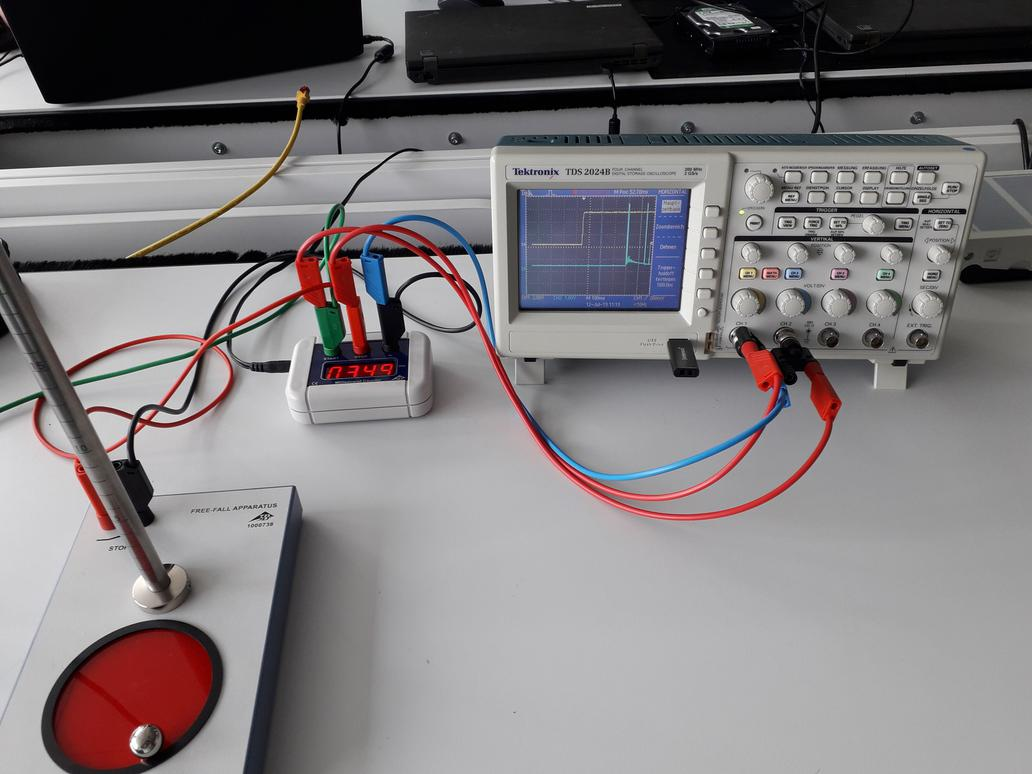
\includegraphics{bilder/Aufbau_Detail_ff.jpg}
	\caption{Anschluss von Digital-Zähler und Oszilloskop}
	\label{AnschlussOsDz}
\end{figure}



\subsection{Versuchsdurchführung}

Die Fallzeiten werden für verschiedene Höhen von 10 bis 90 cm in Schritten von 10 cm durchgeführt. Dabei werden für jede Höhe 10 Zeitmessungen mit dem Digitalzähler und eine Messung mit dem Oszilloskop durchgeführt. Das Oszilloskop wird dabei auf Single Seq eingestellt und auf die steigende Flanke des Startsignals getriggert. Das Triggerlevel liegt dabei bei 620 mV. Um eine Startgeschwindidkeit der Kugel zu vermeiden, wird der Auslösebügel möglichst feinfühlig betätigt. Es werden stets alle Messungen für eine Höhe durchgeführt, ehe die Höhe verstellt wird. Bei der Höheneinstellung wird versucht mit der oberen Bohrungskante der Startkonsole genau den Strich der Säulenskala zu treffen.


\subsection{Versuchsauswertung}

\subsubsection{Messung mit dem Digitalzähler}

Für die Höhenmessung ist entscheidend mit welcher Genauigkeit man den Skalenstrich trifft. Dabei wird die Unsicherheit auf $\sigma_s = 1 \, \mathrm{mm}$ geschätzt. Mit dem Digitalzähler ergaben sich die Messsungen aus Tabelle \ref{tableDz}.

\begin{table}[h]
\begin{center}
\begin{tabular}{c|r|r|r|r|r|r|r|r|r}
$s$ / cm & 10 & 20 & 30 & 40 & 50 & 60 & 70 & 80 & 90 \\
\hline
$t$ / ms & 140 & 200 & 245 & 284 & 318 & 348 & 376 & 403 & 427 \\
         & 140 & 200 & 246 & 284 & 318 & 348 & 377 & 403 & 427 \\
	 & 140 & 200 & 246 & 284 & 318 & 348 & 376 & 403 & 427 \\
	 & 141 & 200 & 246 & 284 & 318 & 348 & 377 & 403 & 427 \\
	 & 141 & 200 & 246 & 284 & 318 & 348 & 377 & 402 & 407 \\
	 & 141 & 200 & 245 & 284 & 318 & 348 & 376 & 402 & 427 \\
	 & 141 & 200 & 246 & 284 & 318 & 348 & 376 & 402 & 427 \\
	 & 141 & 200 & 245 & 284 & 318 & 348 & 376 & 402 & 427 \\
	 & 141 & 200 & 245 & 284 & 318 & 348 & 376 & 403 & 427 \\
	 & 141 & 200 & 246 & 284 & 318 & 348 & 376 & 402 & 427 \\
\hline
$\bar t$ / ms & 140.7 & 200.0 & 245.6 & 284.0 & 318.0 & 348.0 & 376.3 & 402.5 & 427.0
\end{tabular}
\caption{Messreihe mit dem Digitalzähler}
\label{tableDz}
\end{center}
\end{table}

Aufgrund der geringen statistischen Effekte in der Messreihe werden statistische Unsicherheiten vernachlässigt und die Unsicherheit aufgrund der zeitlichen Auflösung des Zählers unter Annahme einer Gleichverteilung zu $\sigma_t = 1/\sqrt{12} \, \mathrm{ms} \approx 0.29 \, \mathrm{ms}$ bestimmt. Wir führen nun mit den berechneten Mittelwerten eine Regression durch. Da in unserem Experiment die Anfangsgeschwindigkeit $v_0$ der Kugel vernachlässigbar sein sollte, haben wir einen linearen Zusammenhang zwischen $s$ und $t^2$. Es gilt
$$s(t) = s_0 + mt^2.$$
Deswegen führen wir eine lineare Regression von $s$ über $t^2$ durch. Dazu berechnen wir zunächst die Werte für $t^2$ und bestimmen den Fehler dieser gemäß
$$\sigma_{t^2} = 2|t|\sigma_t.$$
Die Ergebnisse der Regression sind in Tabelle \ref{tableReg1} aufgelistet.

\begin{table}[h!]
\begin{center}
\begin{tabular}{c|c|c}
$m$ & $s_0$ & $\chi^2/n_{df}$ \\
\hline
$(4.9221 \pm 0.0084) \, \mathrm m / \mathrm s^2$ & $(0.0028 \pm 0.0009) \, \mathrm m$ & $0.14$
\end{tabular}
\caption{Ausgabe der Regression}
\label{tableReg1}
\end{center}
\end{table}

\begin{figure}[h!]
	\centering
	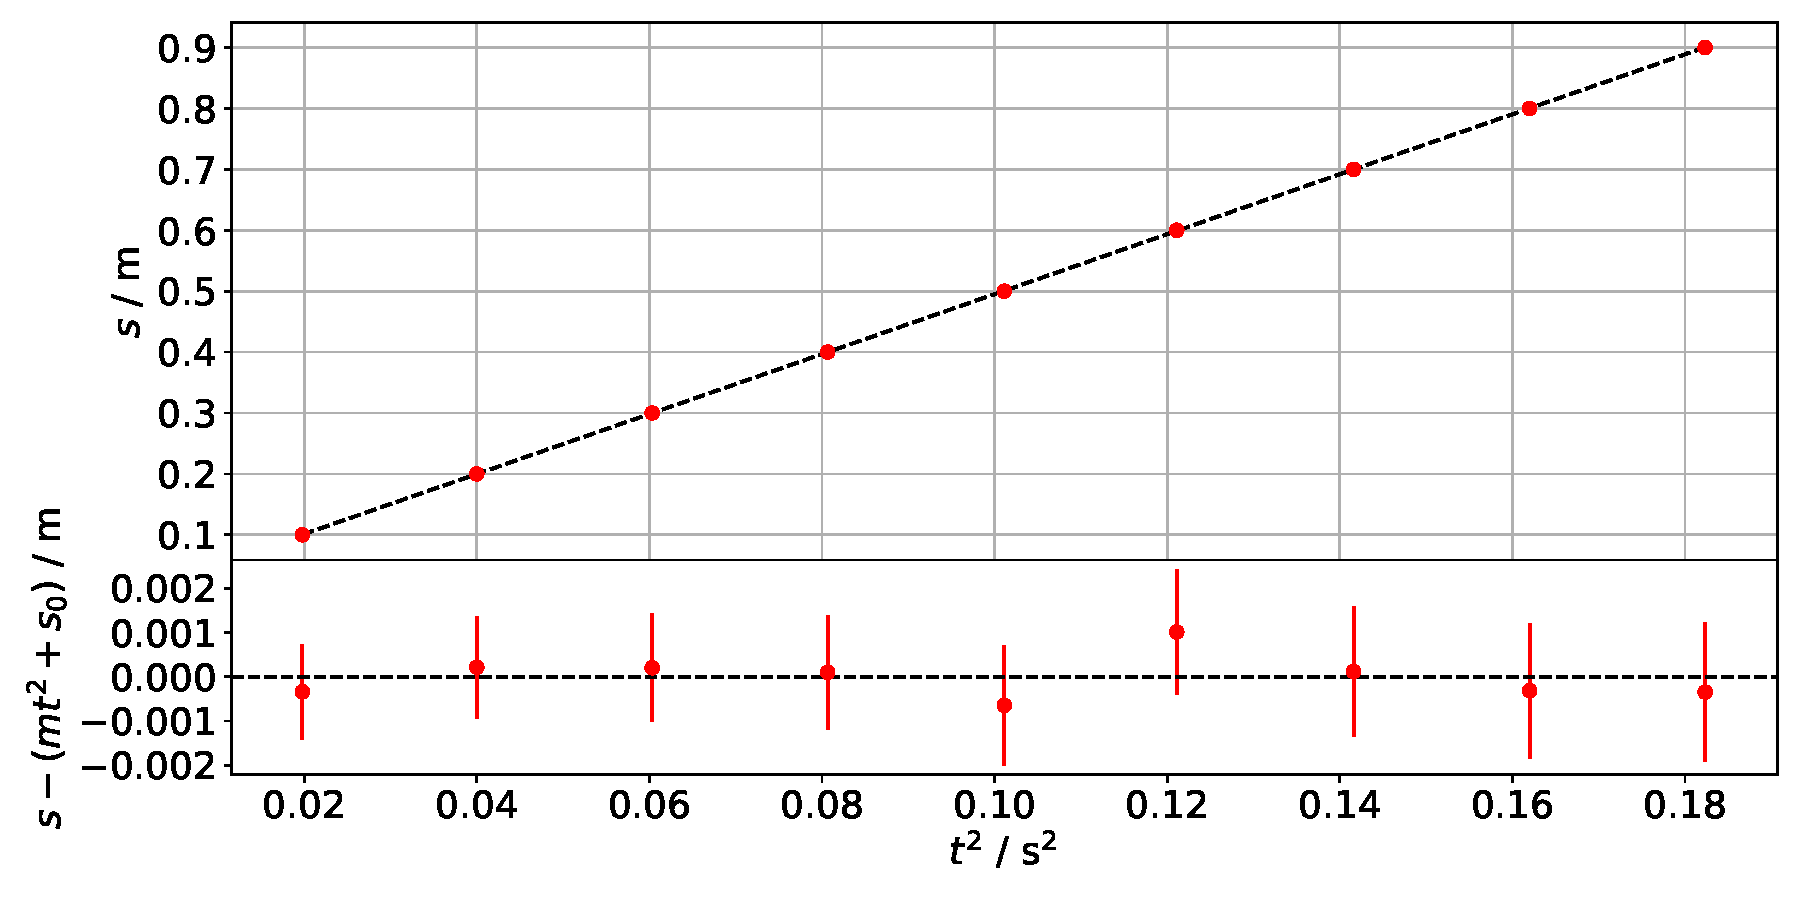
\includegraphics[width=\textwidth]{plots/regression_fF1.pdf}
	\caption{Residuenplot für den Digitalzähler}
	\label{ResDz}
\end{figure}

Der sehr schlechte Wert für $\chi^2/n_{df}$ spiegelt sich auch im Residuengraph wieder (Abb. \ref{ResDz}), wo alle Fehlerbalken deutlich die Nulllinie treffen. Zusammen führt dies zu dem Schluss, dass die Fehlerabschätzungen für $s$ und $t$ zu grob sind. Da wir jedoch keine bessseren Abschätzungen machen können, führen wir noch eine alternative Auswertung der Daten durch. Dazu berechnen wir für je zwei benachbarte Datenpunkte in unserem $s-t^2$-Diagramm die Steigung, wobei der erste Wert nicht verwendet wird. Für die Steigung gilt
$$m = \frac{s_{i+1}-s_i}{t_{i+1}^2-t_{i}^2}.$$
Dies liefert uns vier Schätzungen für die Steigung. Die Fehler werden mit einer Gaußschen Fehlerfortplanzung bestimmt. Diese liefert uns
$$\frac{\sigma_m^2}{m^2} = \frac{2}{(s_{i+1}-s_i)^2}\cdot\sigma_s^2 + \frac{4(t_{i+1}^2 + t_i^2)}{(t_{i+1}^2-t_i^2)^2}\cdot\sigma_t^2.$$
Anschließend werden die vier Steigungswerte mit ihren Unsicherheiten gewichtet gemittelt und innerer und äußerer Fehler des Mittelwertes bestimmt. Die Ergebnisse dieser Kalkulation sind in Tabelle \ref{tableAltAus} zu sehen. 

\begin{table}[h!]
\begin{center}
\begin{tabular}{c|c}
$m_1$ & $(4.921 \pm 0.083) \, \mathrm m / \mathrm s^2$ \\ 
$m_2$ & $(4.886 \pm 0.091) \, \mathrm m / \mathrm s^2$ \\
$m_3$ & $(4.879 \pm 0.099) \, \mathrm m / \mathrm s^2$ \\
$m_4$ & $(4.921 \pm 0.109) \, \mathrm m / \mathrm s^2$ \\
\hline
$\bar m$ & $4.902 \, \mathrm m / \mathrm s^2$ \\
$\sigma^{in}_{\bar m}$ & $0.047 \, \mathrm m / \mathrm s^2$ \\
$\sigma^{au}_{\bar m}$ & $0.011 \, \mathrm m / \mathrm s^2$
\end{tabular}
\caption{Alternative Auswertung der Daten}
\label{tableAltAus}
\end{center}
\end{table}
Aus dem Wert der Steigung ergibt sich dann die Schätzung für die Erdbeschleunigung
$$g = (9.80 \pm 0.09) \, \mathrm m / \mathrm s^2 .$$

\subsubsection{Messung mit dem Oszilloskop}

Die Messungen mit dem Oszilloskop sind in Tabelle \ref{tableOs} aufgeführt. 
\begin{table}[h!]
\begin{center}
\begin{tabular}{c|r|r|r|r|r|r|r|r|r}
$s$ / cm & 10 & 20 & 30 & 40 & 50 & 60 & 70 & 80 & 90 \\
\hline
$t$ / ms & 140.8 & 200.0 & 245.2 & 283.8 & 318.2 & 348.4 & 376.6 & 402.7 & 427.2 \\
\end{tabular}
\caption{Messreihe mit dem Oszilloskop}
\label{tableOs}
\end{center}
\end{table}

Die Genauigkeit der Zeitmessung mit dem Oszilloskop wird auf $\sigma_t = 0.1 \, \mathrm{ms}$ geschätzt. Wir führen wieder ein lineare Regression von $s$ über $t^2$ durch. Die Ergebnisse befinden sich in Tabelle \ref{tableReg2}.

\begin{table}[h!]
\begin{center}
\begin{tabular}{c|c|c}
$m$ & $s_0$ & $\chi^2/n_{df}$ \\
\hline
$(4.9123 \pm 0.0066) \, \mathrm m / \mathrm s^2$ & $(0.0035 \pm 0.0007) \, \mathrm m$ & $0.5$
\end{tabular}
\caption{Ausgabe der Regression}
\label{tableReg2}
\end{center}
\end{table}

Der Wert für $\chi^2/n_{df}$ deutet wieder auf eine zu grobe Fehlerabschätzung hin. Dies zeigt sich auch wieder im Residuenplot (Abb. \ref{ResOz}), wo fast alle Fehlerbalken die Nulllinie treffen.
\begin{figure}[h!]
	\centering
	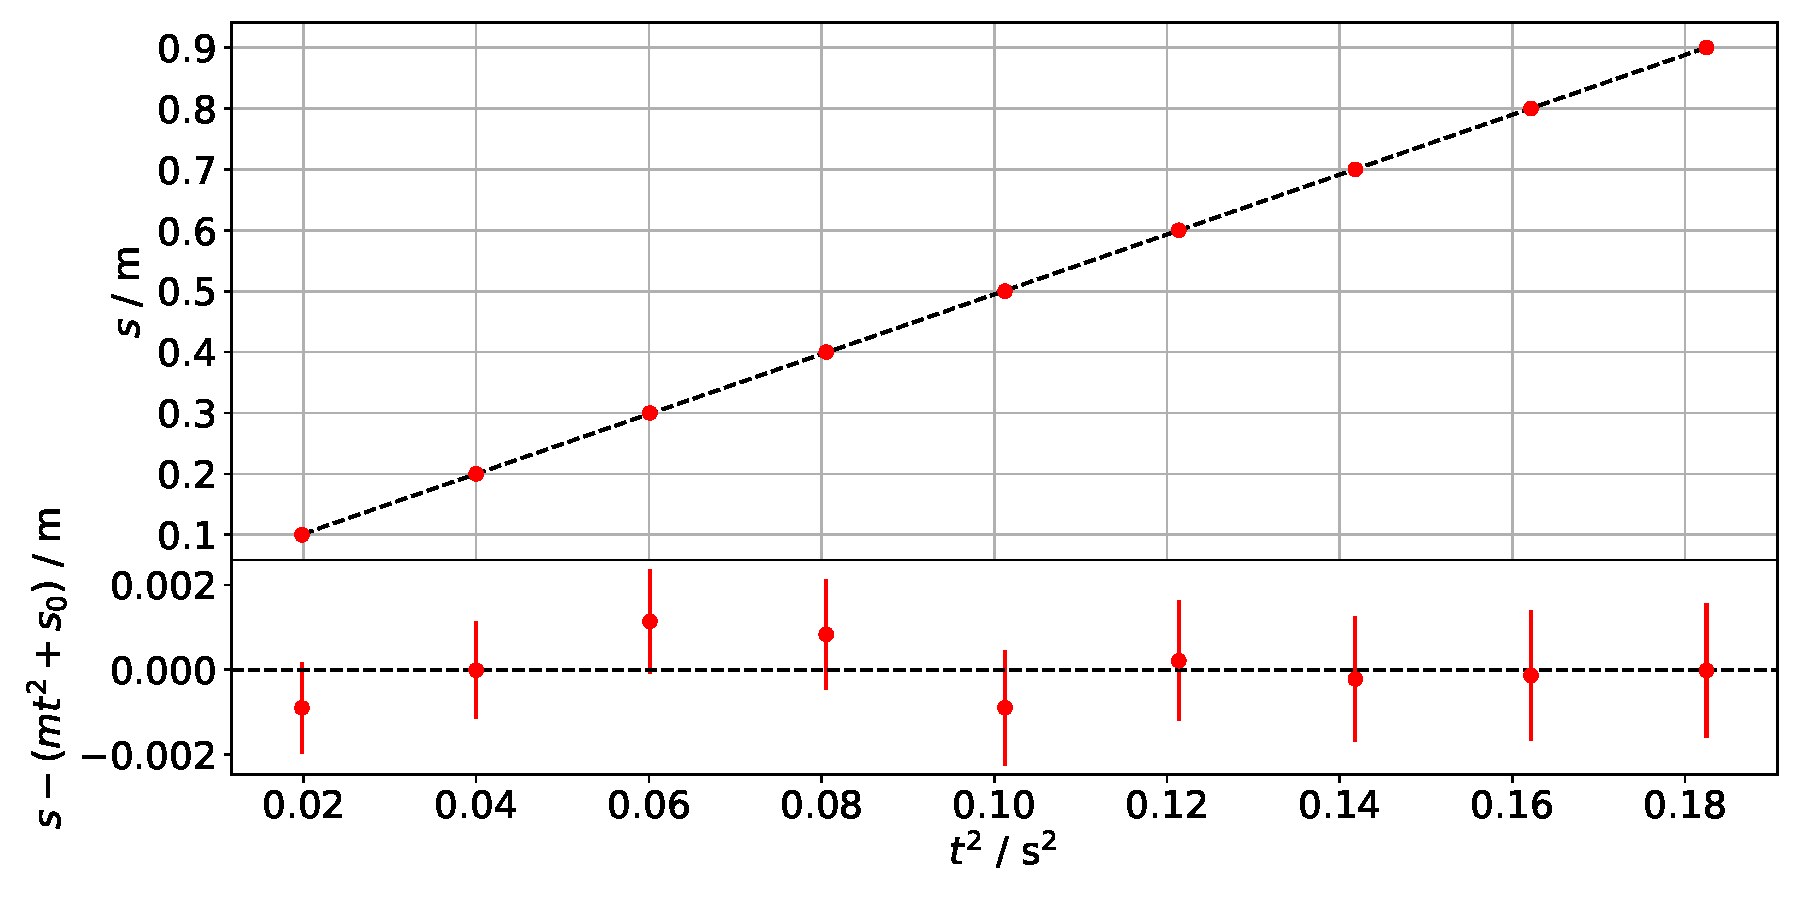
\includegraphics[width=\textwidth]{plots/regression_fF2.pdf}
	\caption{Residuenplot für das Oszilloskop}
	\label{ResOz}
\end{figure}
Trotzdessen verwenden wir die Ergebnisse dieser Regression, da die Anpassung deutlich besser ist, als im Falle des Digitalzählers. Aus der Steigung ermitteln wir folgende Schätzung für die Erdbeschleunigung
$$g = (9.824 \pm 0.013) \, \mathrm m / \mathrm s^2 .$$


\subsection{Fazit}

Wir haben nun zwei Schätzungen für die Erdbeschleunigung $g$ ermittelt. Wie im Fazit des zweiten Versuchs erläutert, verwenden wir als Literaturwert für die Erbeschleunigung in Aachen $g_L = 9.811 \, \mathrm m / \mathrm s^2$. 
Zur Bewertung der beiden Ergebnisse berechnen wir
\begin{align*}
\frac{|g_L-g_{Dz}|}{\sigma_{g_{Dz}}} &= 0.12 \\
\frac{|g_L-g_{Os}|}{\sigma_{g_{Os}}} &= 1
\end{align*}
In beiden Fällen liegen wir somit im $1\sigma$-Intervall. Zur Überprüfung der Übereinstimmung der beiden Werte untereinander berechnen wir noch
$$\frac{|g_{Os}-g_{Dz}|}{\sqrt{\sigma_{g_{Dz}}^2 + \sigma_{g_{Os}}^2}} \approx 0.03 \ll 1.$$
Die beiden Werten stimmen also im Rahmen der Unsicherheiten sehr gut überein. 


\newpage


\section{Erdbeschleunigung mit dem Pendel}


\subsection{Versuchsbeschreibung}

In diesem Experiment wird die Schwingung eines physikalischen Pendels untersucht, um die Erdbeschleunigung $g$ zu bestimmen. Die Schwingungsgleichung für das physikalische Pendel lautet
$$J \ddot \varphi = - mgl_s \sin(\varphi)\text{.}$$
Dabei ist $J$ das Gesamtträgheitsmoment des Pendels und $l_s$ der Abstand vom Aufhängepunkt zum Schwerpunkt des Pendels, sowie $\varphi$ der Auslenkwinkel aus der Ruhelage. Auf der rechten Seite der Gleichung steht das rücktreibende Drehmoment, welches durch die Gravitationskraft hervorgerufen wird. Für kleine Winkel, bei denen $\sin(\varphi) \approx \varphi$ näherungsweise gilt, ergibt sich die lineare, homogene Differentialgleichung zweiter Ordnung
$$\ddot \varphi = -\frac{mgl_s}J \varphi\text{.}$$
Diese Gleichung hat die allgemeine Lösung
$$\varphi(t) = A\cdot \cos(\omega t)+ B\cdot \sin(\omega t)\text{.}$$
Die Kreisfrequenz $\omega$ dieser Schwingung ist gegeben durch
$$\omega^2 = \frac{mgl_s}J\text{.}$$
Da das Trägheitsmoment $J$ des Pendels schwierig zu bestimmen ist, umgehen wir dieses Problem. Das betrachtete Pendel besteht aus einem Winkelaufnehmer-Profil, der Pendelstange und einem zylindrischen Pendelkörper.

\begin{figure}[h]
	\centering
	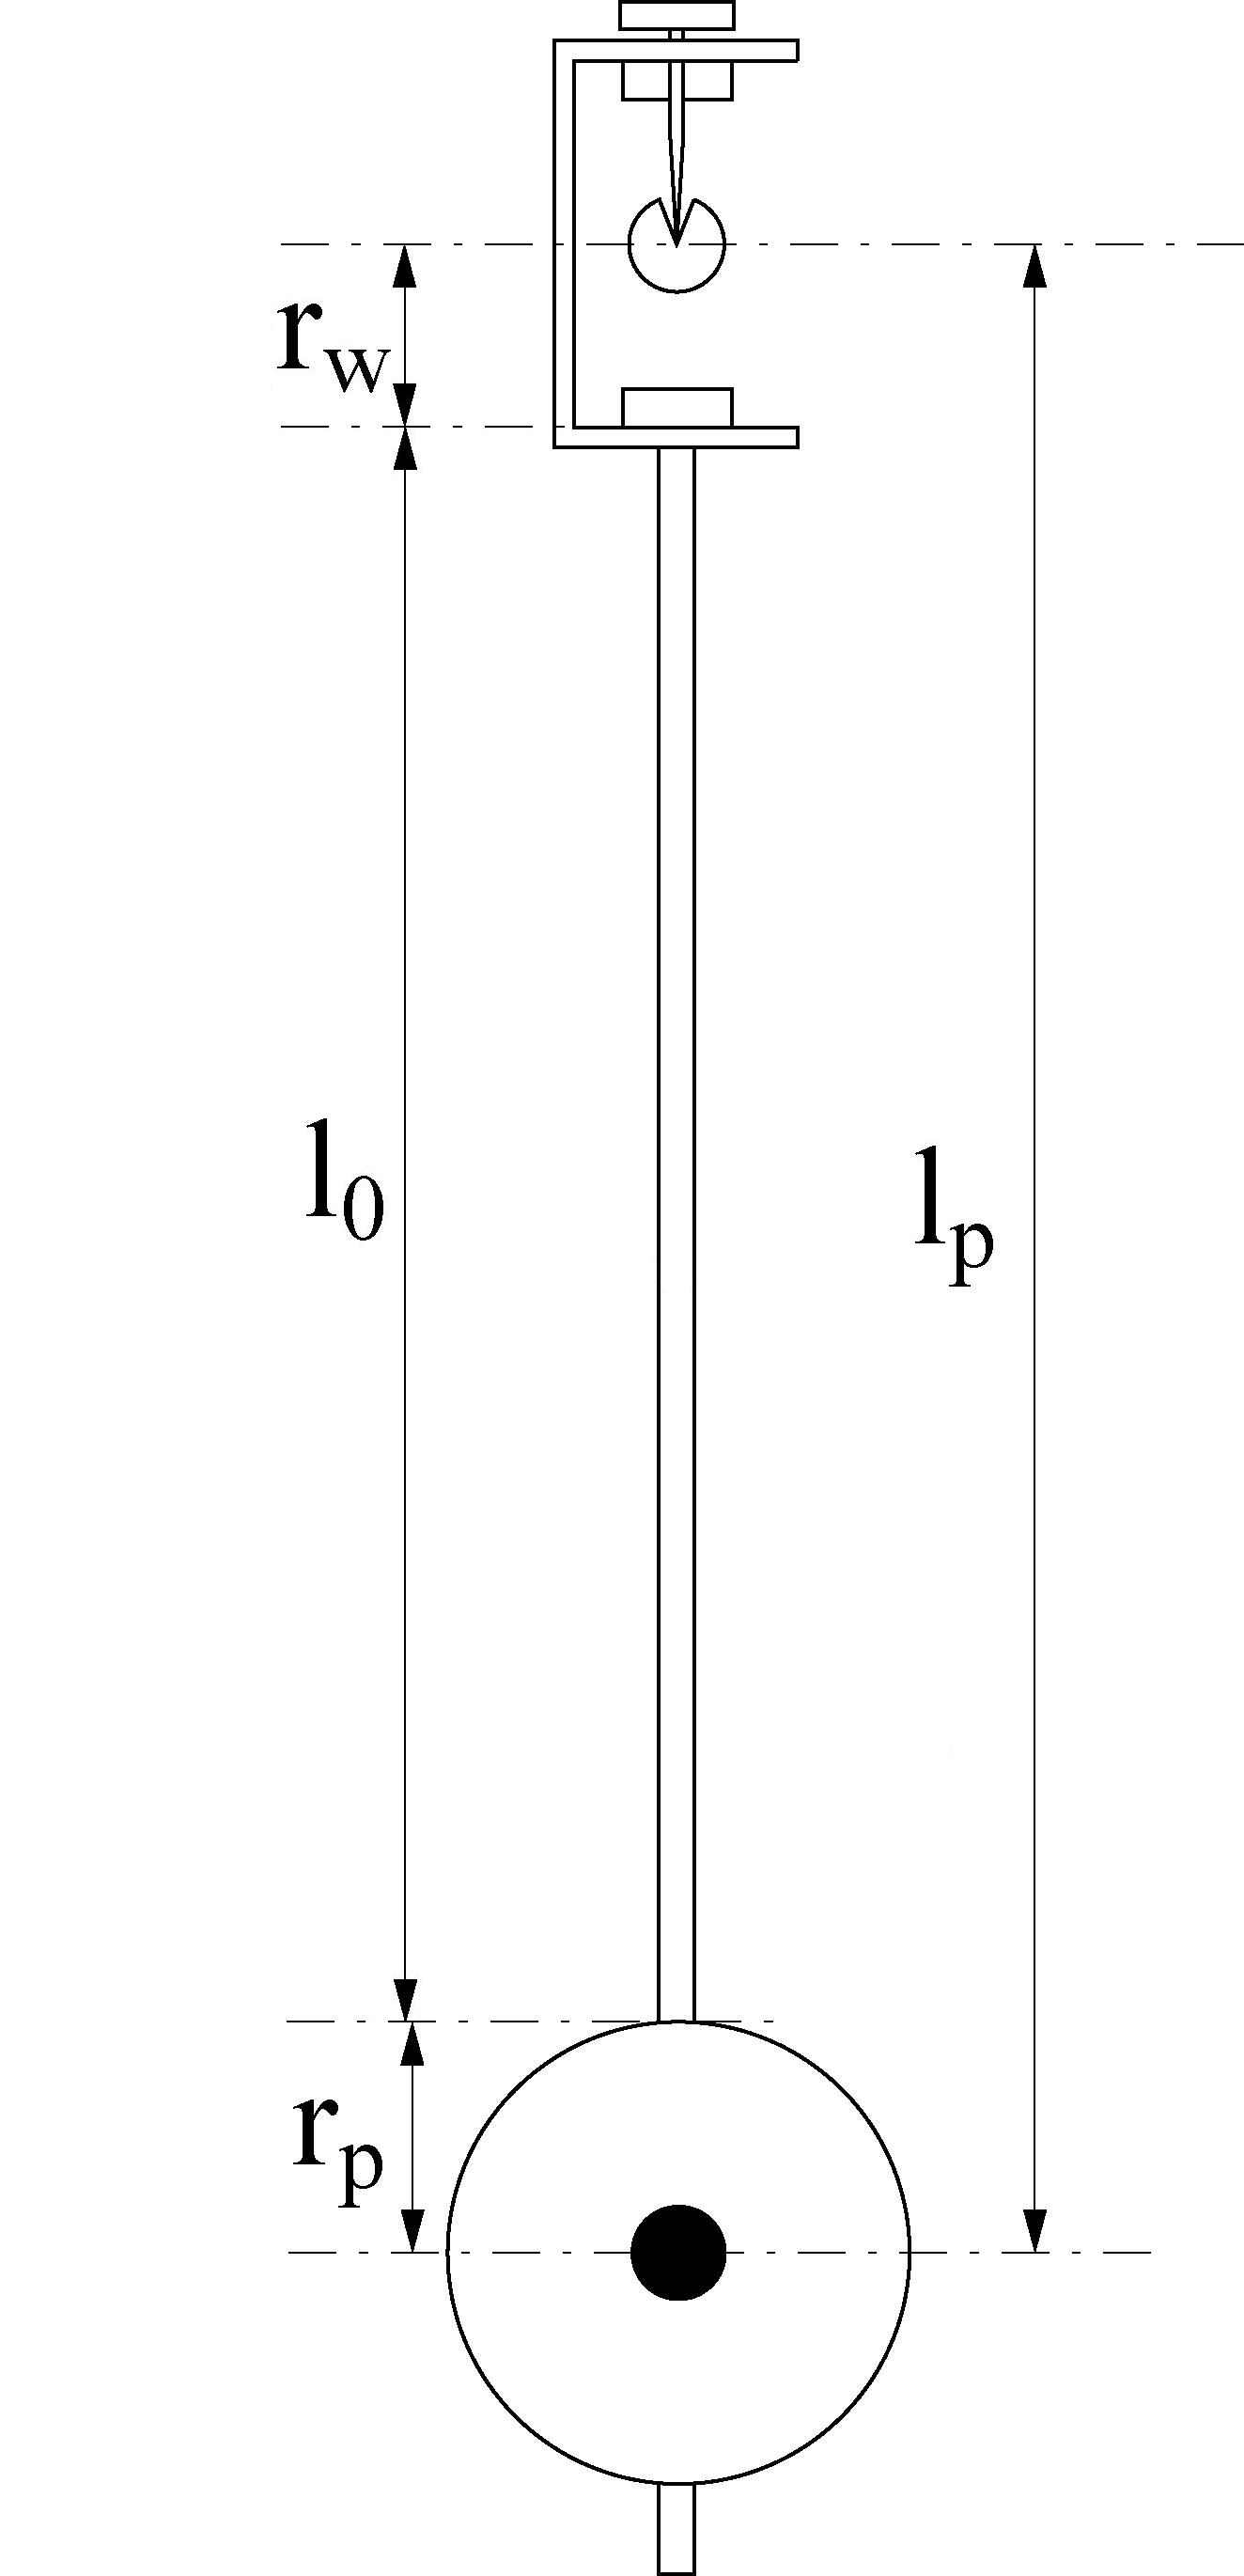
\includegraphics[scale=0.15]{bilder/Pendel_Zeichnung_be.jpg}
	\caption{Schematische Zeichung des Pendels}
\end{figure}

Wir bestimmen zunächst die Schwingungsfrequenz $\omega_{st}$ der Stange. Anschließend wird der Pendelkörper so an der Stange angebracht, dass das Pendel mit Pendelkörper und Stange die gleiche Schwingungsfrequenz hat wie die Stange allein. Sind $D_{st}$ und $D_p$ die maximalen Rückstellmomente von Stange und Pendelkörper und $J_{st}$ und $J_p$ die entsprechenden Trägheitsmomente, so gilt für die Schwingungfrequenz der Stange allein
$$\omega_{st}^2 = \frac{D_{st}}{J_{st}}\text{.}$$
Für den Pendelkörper allein gilt analog
$$\omega_p^2 = \frac{D_p}{J_p}\text{.}$$
Da die Rückstellmomente und die Trägheitsmomente additiv sind, ergibt sich die Frequenz des physikalischen Pendels mit Stange und Pendelkörper zu
$$\omega^2 = \frac{D_{st} + D_p}{J_{st} + J_p} = \omega_{st}^2 \frac{1+\frac{D_p}{D_{st}}}{1+\frac{J_p}{J_{st}}}\text{.}$$
Ist der Pendelkörper nun so eingestellt, dass $\omega = \omega_{st}$, so muss $\frac{D_p}{D_{st}} = \frac{J_p}{J_{st}}$ gelten. Daraus erhält man schließlich
$$\omega_p = \omega_{st} = \omega\text{.}$$
Das Pendel lässt sich so betrachten als bestünde es nur aus dem Pendelkörper. Mit dem Trägheitsmoment des geometrisch einfachen Pendelkörpers und dem Satz von Steiner ergibt sich
$$J_p = \frac 12 m_p r_p^2 + m_pl_p^2\text{.}$$
Damit lässt sich nun die Kreisfrequenz des Pendels ausdrücken
$$\omega^2 = \omega_p^2 = \frac{D_p}{J_p} = \frac{m_pgl_p}{\frac 12 m_pr_p^2+m_pl_p^2}\text{.}$$
Durch Umformen folgt schließlich die Formel für die Erdbeschleunigung
$$g = \omega^2l_p \left( 1 + \frac 12 \frac{r_p^2}{l_p^2} \right)\text{.}$$
Durch Messung des Radius $r_p$ und der Länge $l_p$, sowie der Periodendauer $T = \frac{2\pi}{\omega}$, lässt sich somit die Erdbeschleunigung bestimmen.

\subsection{Versuchsaufbau und -durchführung}


\subsection{Auswertung}
Nach der Kalibrierung der Winkelgeschwindigkeit wurden folgende Längen für das Pendel mit Pendelkörper gemessen:

\begin{table}[H]
\centering
\begin{tabular}{c|c|c}
$r_w$ & $l_0$ & $r_p$ \\
\hline
$2.535\text{cm} \pm 0.005\text{cm}$ & $61.5\text{cm}\pm 0.069\text{cm}$ & $3.998\text{cm} \pm 0.003\text{cm}$
\end{tabular}
\caption{Ergebnisse der Längenmessungen}
\end{table}

Das ergibt eine Pendellänge $l_p = r_w + l_0 + r_p = 68.033 \text{cm}$ mit einem Fehler von $\sigma_{l_p} = 0.07 \text{cm}$. Aus den mit dem Sensor-Cassy aufgenommenen Rohdaten ergeben sich folgende Zeitpunkte an denen das Pendel mit bzw. ohne Pendelkörper die $n$-te maximale Auslenkung annimmt:

\begin{table}[H]
\centering

\begin{adjustbox}{width=\textwidth}
\begin{tabular}{c|cccccccccc}
Schwingung & 1 & 10 & 20 & 30 & 40 & 50 & 60 & 70 & 80 & 90 \\
\hline
Zeitpunkt (Pendelkörper) [s] & 0.48 & 15.38 & 31.94 & 48.48 & 65.04 & 81.56 & 98.11 & 114.68 & 131.28 & 147.84 \\
Zeitpunkt (nur Stange) [s] & 1.5 & 16.44 & 33.01 & 49.59 & 66.14 & 82.73 & 99.32 & 115.86 & 132.46 & 149.05
\end{tabular}
\end{adjustbox}
\end{table}

\begin{table}[H]
\centering
\begin{adjustbox}{width=\textwidth}
\begin{tabular}{c|cccccccccc}
Schwingung & 100 & 110 & 120 & 130 & 140 & 150 & 160 & 170 & 180 & 190 \\
\hline
Zeitpunkt (Pendelkörper) [s] & 164.36 & 180.9 & 197.46 & 214.02 & 230.56 & 247.12 & 263.68 & 280.22 & 296.8 & 313.34 \\
Zeitpunkt (nur Stange) [s] & 165.64 & 182.18 & 198.8 & 215.34 & 231.92 & 248.47 & 265.08 & 281.62 & 298.23 & 314.83
\end{tabular}
\end{adjustbox}
\end{table}

\begin{figure}[h]
	\centering
	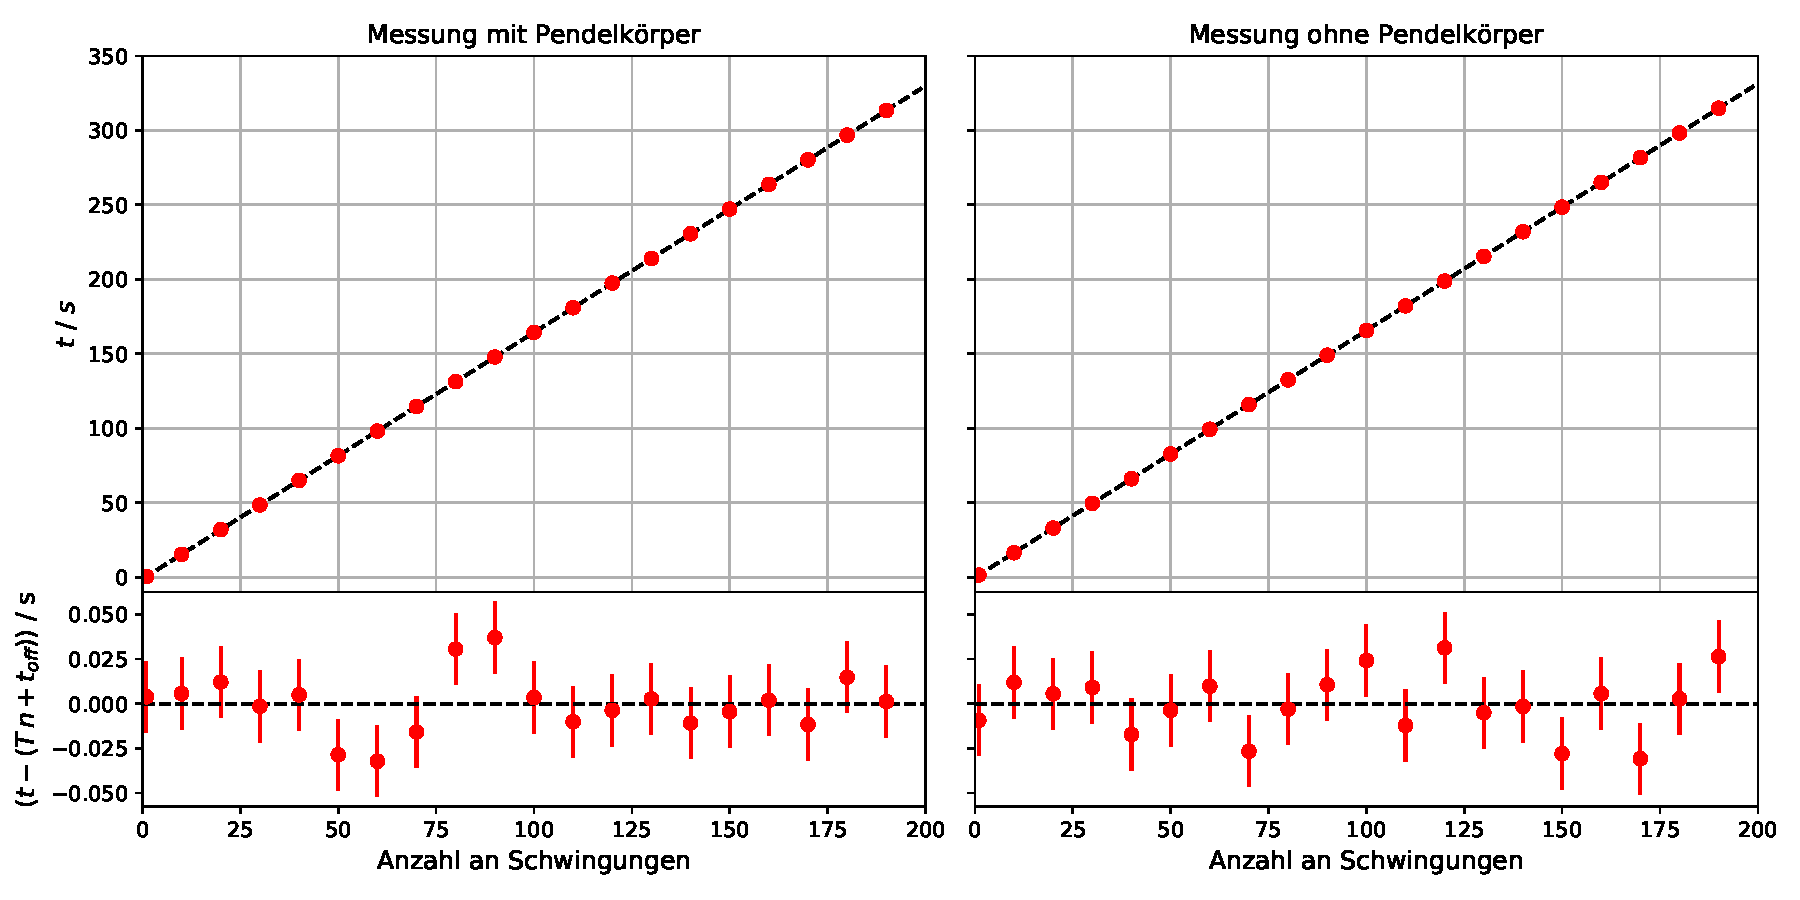
\includegraphics[width = \textwidth]{plots/regression.pdf}
	\caption{Regression und Residuenplot für Datenpunkte aus dem Versuch mit und ohne Pendelkörper}\label{plot:regression}
\end{figure}

Diese Datenpunkte wurden mit einer Genauigkeit von $\sigma_{t} = 0.02\text{s}$ bestimmt. Eine lineare Regression der Zeitpunkte mit Residuenplot ist in Abbildung \ref{plot:regression} zu sehen und liefert eine Periodendauer von $T_p = 1.65536 \text{s} \pm 7\cdot 10^{-5} \text{s}$ ($\chi^2 = 0.73$) bzw. $T_{st} = 1.65764 \text{s} \pm 7\cdot 10^{-5}\text{s}$ ($\chi^2 = 0.80$). Die $\chi^2$-Werte sind dabei zufriedenstellend. Mit $\omega = \frac{2\pi}{T}$ führt das zu den Kreisfrequenzen $\omega_p = 3.79566\, \text{Hz}\, \pm 0.00018\, \text{Hz}$ und $\omega_{st} = 3.79043\, \text{Hz} \,\pm 0.00018\, \text{Hz}$. Dabei ist der Fehler in $\omega$ nach Gaußscher Fehlerfortpflanzung durch
$$ \sigma_\omega = \left| \frac{\partial \omega (T)}{\partial T} \sigma_T \right | = \frac{2\pi}{T^2} \sigma_T $$
gegeben.

\begin{figure}[h]
	\centering
	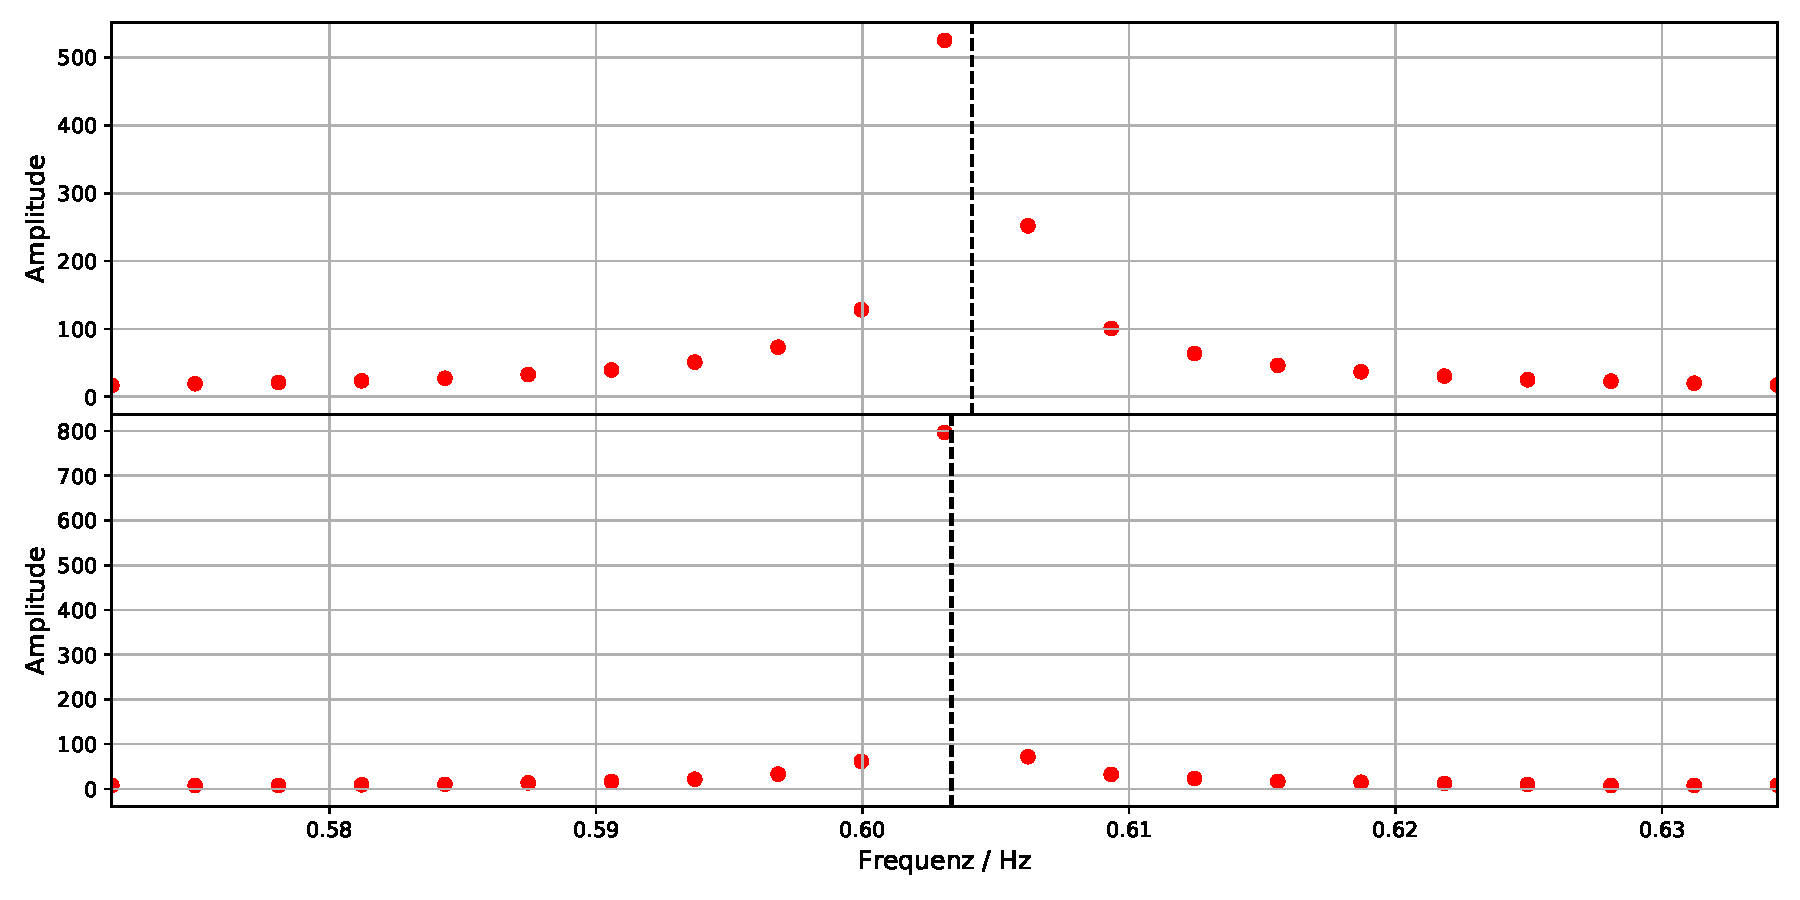
\includegraphics[width = \textwidth]{plots/fft.pdf}
	\caption{FFT der Rohdaten und Peakanalyse - oben mit Pendelkörper und unten ohne Pendelkörper}\label{plot:fft}
\end{figure}

Eine Analyse der Schwingung mit Hilfe einer FFT liefert die Ergebnisse $\omega_p = 2\pi f_p =  3.79567 \text{Hz}$ und $\omega_{st} = 2\pi f_s = 3.79093 \text{Hz}$ und passt somit zu den Werten, die die Regressionsanalyse liefert. Der Plot davon ist in Abbildung \ref{plot:fft} dargestellt. Aufgrund der mangelnden Fehleranalyse wird ausschließlich mit den Werten aus der Regressionsanalyse weitergearbeitet. \\
Aus den bisher bestimmten Größen ergibt sich eine Erdbeschleunigung von 
$$ g = \omega_p^2l_p \left( 1 + \frac 12 \frac{r_p^2}{l_p^2} \right) = 9.8184 \frac{\text{m}}{\text{s}^2}\text{.}$$
Um die Fehlerbetrachtung durchzuführen, wird $g$ als Funktion in $\omega_p$, $l_p$ und $r_p$ betrachtet. Wie in der Praktikumsanleitung für den Versuch diskutiert, kann der Fehler in $r_p$ vernachlässigt werden. Die relative Abweichung von Schwingung mit und ohne Pendelkörper beträgt
$$\frac{\lvert \omega_p - \omega_{st}\rvert}{\omega_p} = 0.0014$$
und wird daher ebenfalls vernachlässigt. Für die relevanten partiellen Ableitungen von $g$ gilt
$$\frac{\partial g}{\partial \omega_p} = 2\omega_p l_p \left(1+\frac 12 \frac{r_p^2}{l_p^2}\right) \text{ und}$$
$$\frac{\partial g}{\partial l_p} = \omega_p^2 \left(1-\frac 12 \frac{r_p^2}{l_p^2}\right)\text{.}$$
Das ergibt einen Fehler von
$$\sigma_g = 0.010 \frac{m}{s^2}\text{.}$$

\subsection{Fazit}
Die Physikalisch-Technische Bundesanstalt gibt in einer ihrer Publikationen\footnote{\url{https://www.ptb.de/cms/fileadmin/internet/fachabteilungen/abteilung_1/1.1_masse/1.15/gravzonen.pdf}} die Erdbeschleunigung für die Stadt Brüssel mit $g = 9.811 \frac{\text{m}}{\text{s}^2}$ an. Da Aachen und Brüssel näherungsweise den gleichen Breitengrad haben (Brüssel: 50.84°, Aachen: 50.78°), wird dieser Wert als Literaturwert verwendet. \\
Der Literaturwert liegt im $1\sigma$-Intervall des im Experiment bestimmten Wert $9.818 \frac{\text{m}}{\text{s}^2} \pm 0.010 \frac{\text{m}}{\text{s}^2}$ und somit innerhalb der Fehlertoleranz. Der schwerwiegendste Fehler im Experiment wurde durch die Messung der Länge $l_0$ gemacht. 


\end{document}
